% The code is quite messy !!!

\documentclass[tikz, border=10pt]{standalone}

\begin{document}

    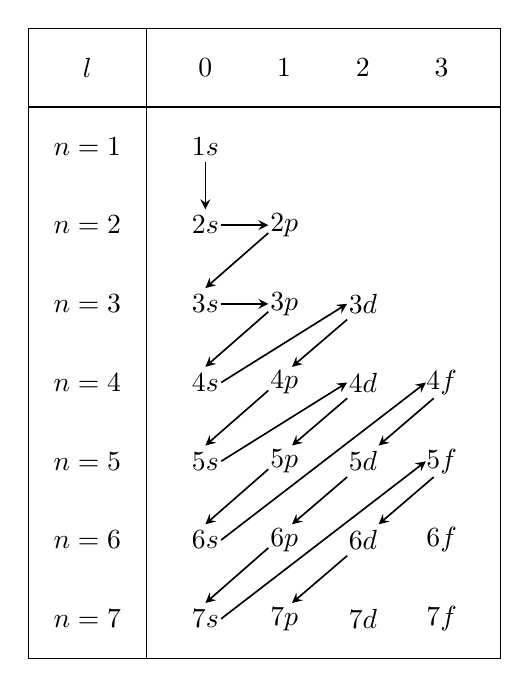
\begin{tikzpicture}
        % Style pour les flèches
        \tikzstyle{arrow} = [semithick,->,>=stealth]

        % Ajout des étiquettes pour n (niveau) à gauche
        \foreach \n in {1,..., 7}{
            \node at (-1.5,-\n+1) {$n=\n$};
        }
        % Ajout des étiquettes pour l (valeur de sous-couche) en haut
        \node at (-1.5,1) {$l$};
        \foreach \n in {0,...,3}{
        \node at (\n,1) {$\n$};
        }

        % Dessin des lignes de séparation horizontales pour n
        \draw[] (-2.25,1.5) -- (3.75,1.5);
        \draw[] (-2.25,0.5) -- (3.75,0.5);
        \draw[] (-2.25,-6.5) -- (3.75,-6.5);

        % Dessin des lignes de séparation verticales pour l
        \draw[] (-2.25,1.5) -- (-2.25,-6.5);
        \draw[] (-0.75,1.5) -- (-0.75,-6.5);
        \draw[] (3.75,1.5) -- (3.75,-6.5);

        % Positionnement des sous-couches sans contour
        \foreach \n in {1,...,7}{
        \node at (0,-\n+1) {$\n s$};}
        \foreach \n in {2,...,7}{
        \node at (1,-\n+1) {$\n p$};}
        \foreach \n in {3,...,7}{
        \node at (2,-\n+1) {$\n d$};}
        \foreach \n in {4,...,7}{
        \node at (3,-\n+1) {$\n f$};}

        % Dessin des flèches suivant la règle de Klechkowski
        \draw[arrow] (0,-0.2) -- (0,-0.8);       % 1s -> 2s
        \draw[arrow] (0.2,-1) -- (0.8,-1);       % 2s -> 2p
        % fleches p à s
        \foreach \n in {1,...,5}{
        \draw[arrow] (0.8,-\n-0.1) -- (0,-\n-0.8);}
        % fleche p à d
        \foreach \n in {2,...,5}{
        \draw[arrow] (1.8,-\n-0.2) -- (1.1,-\n-0.8);}
        \draw[arrow] (0.2,-2) -- (0.8,-2);       % 3s -> 3p
        \draw[arrow] (0.2,-3) -- (1.8,-2);       % 4s -> 3d
        \draw[arrow] (0.2,-4) -- (1.8,-3);       % 5s -> 4d
        \draw[arrow] (0.2,-5) -- (2.8,-3);       % 6s -> 4f
        \draw[arrow] (2.9,-3.2) -- (2.2,-3.8);   % 4f -> 5d
        \draw[arrow] (0.2,-6) -- (2.8,-4);       % 7s -> 5f
        \draw[arrow] (2.9,-4.2) -- (2.2,-4.8);   % 5f -> 6d
        
    \end{tikzpicture}

\end{document}